% background.tex -- Section 2: Background

\section{Background}
\label{sec:background}

This section describes the architectures and benchmark used in our study: SmolVLA~\cite{shukor2025smolvla} and OpenVLA~\cite{kim2024openvla}, two VLA models with contrasting vision connector designs, and the LIBERO benchmark~\cite{liu2023libero} on which we evaluate closed-loop performance.

\subsection{SmolVLA Architecture}
\label{sec:smolvla_arch}

Vision-Language-Action (VLA) models cast robotic control as conditional generation: given a camera observation and a language instruction, the model predicts a continuous action.
SmolVLA~\cite{shukor2025smolvla} instantiates this paradigm with approximately 450M parameters, organized into a vision encoder, a vision connector, a language model backbone, and an action head.
Figure~\ref{fig:architecture} contrasts the vision pipelines of SmolVLA and OpenVLA, highlighting the connector designs that determine compressibility.

\begin{figure}[t]
\centering
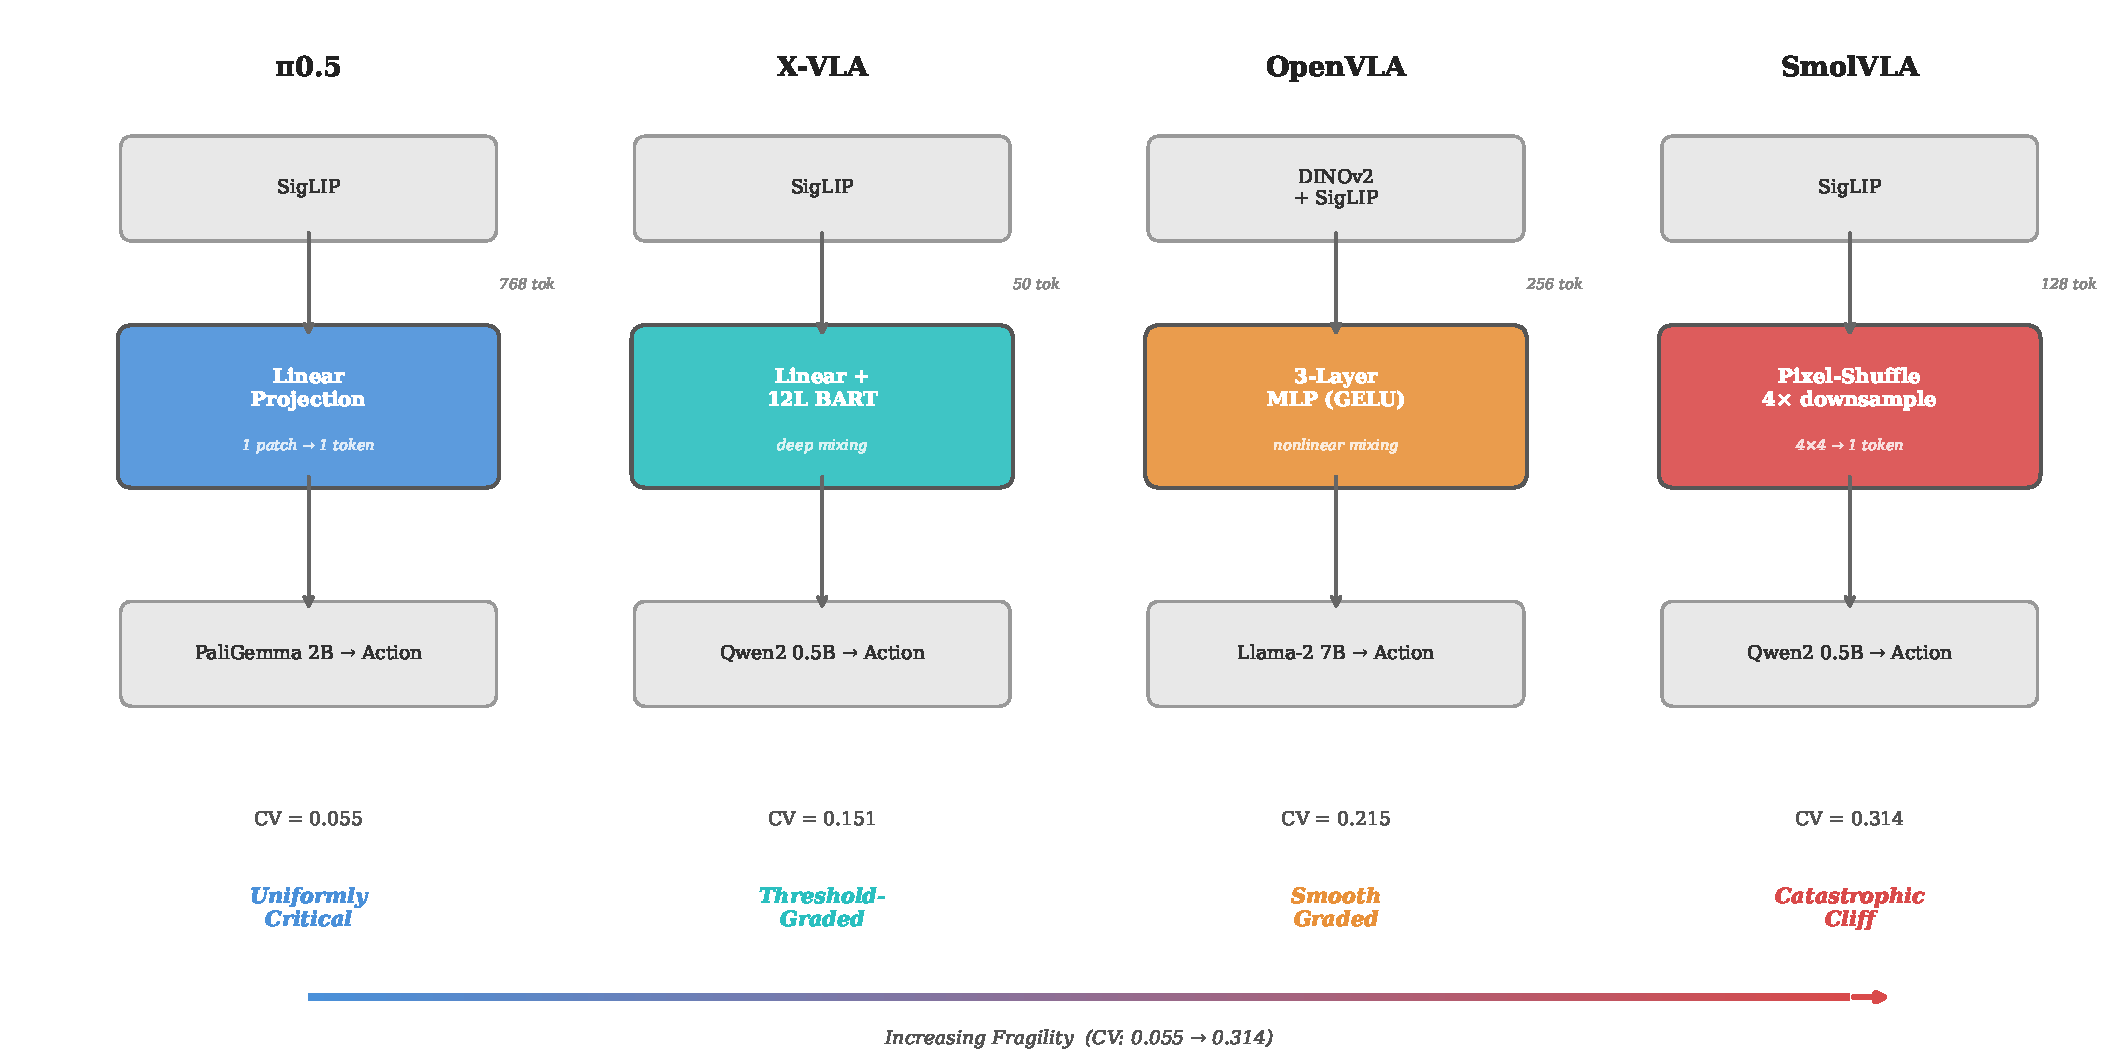
\includegraphics[width=\linewidth]{figures/paper/fig_architecture.pdf}
\caption{Vision connector comparison. \textbf{Left}: SmolVLA applies $4{\times}4$ pixel-shuffle to fold 1024 SigLIP patches into 64 tokens per camera (128 total), creating dense, spatially entangled representations. \textbf{Right}: OpenVLA uses an MLP projector that maps each patch independently, producing 256 tokens with per-token independence. We hypothesize that this architectural difference is the primary factor governing token compressibility: pixel-shuffle tokens resist any form of deletion, while independently projected tokens allow graded pruning.}
\label{fig:architecture}
\end{figure}

\paragraph{Vision encoder.}
SmolVLA uses the Sigmoid Loss for Language-Image Pre-training (SigLIP) encoder~\cite{zhai2023siglip} to process visual input.
SigLIP divides each camera image into non-overlapping spatial patches on a $32 \times 32$ grid, producing 1024 patch tokens per image.
SigLIP does not include a \texttt{[CLS]} aggregation token; there is no single summary representation that pools information across patches.

\paragraph{Pixel-shuffle vision connector.}
Before reaching the language model, the 1024 SigLIP patches pass through a pixel-shuffle connector that applies $4 \times 4$ spatial folding. Each $4 \times 4$ block of spatially adjacent patches is collapsed into a single token by channel concatenation, compressing 1024 patches into 64 tokens per camera image ($16\times$ reduction). An MLP then projects these 64 tokens into the Qwen2-0.5B embedding space. The pixel-shuffle operation is fixed and non-learned; it creates dense tokens where each encodes the full semantic content of 16 contiguous patches. This design choice is central to the cliff-edge phenomenon we report: the spatial folding creates inter-token dependencies that make every token indispensable.

\paragraph{Dual-camera input.}
SmolVLA receives images from two cameras: a wrist-mounted camera and an overhead camera.
Each camera image produces 64 vision tokens after pixel-shuffle, yielding 128 vision tokens total that enter the language model.
The two viewpoints are complementary: the wrist camera captures fine-grained end-effector interactions, while the overhead camera provides a global spatial layout of objects on the workspace.

\paragraph{LLM backbone.}
The Qwen2-0.5B language model~\cite{yang2024qwen2} serves as the central reasoning module.
It receives a concatenated input sequence of 128 projected vision tokens and the tokenized language instruction.
Self-attention across this full sequence allows the model to ground language in visual context and to integrate information across both camera views.

\paragraph{Flow matching action head.}
SmolVLA generates actions through conditional flow matching~\cite{lipman2023flow} rather than autoregressive token prediction.
The action head maps the LLM's output representation to a continuous 7-DoF action vector: three position coordinates, three rotation angles, and one gripper open/close value.
Flow matching learns a vector field that transports a noise distribution to the target action distribution, conditioned on the LLM output.
Any corruption of the vision token input propagates through the full LLM computation into the predicted action.

\subsection{OpenVLA Architecture}
\label{sec:openvla_arch}

OpenVLA~\cite{kim2024openvla} is a 7B-parameter VLA built on the Llama-2 backbone. Its vision pipeline differs from SmolVLA in two respects that are directly relevant to compressibility.

\paragraph{Vision encoder.}
OpenVLA uses a dual encoder combining DINOv2~\cite{oquab2023dinov2} and SigLIP~\cite{zhai2023siglip}. The two encoders produce complementary representations (self-supervised spatial features and language-aligned features) that are concatenated per patch position.

\paragraph{MLP projector.}
Unlike SmolVLA's pixel-shuffle connector, OpenVLA maps vision encoder outputs to the language model through a three-layer MLP projector (GELU activations) that processes each patch token independently. This design preserves per-token independence: the representation of one token carries no implicit dependency on neighboring tokens' presence. The projector produces 256 vision tokens that maintain a one-to-one correspondence with spatial patch locations.

\paragraph{Architectural contrast.}
The key difference for compressibility is the connector design. SmolVLA's pixel-shuffle folds 16 patches into each token, creating dense, entangled representations where removing one token eliminates a $4 \times 4$ spatial region. OpenVLA's MLP projector preserves patch-level granularity, so removing one token discards approximately $1/256$ of the visual field. Model scale (0.5B vs.\ 7B) is a confound that we discuss in Section~\ref{sec:discussion}.

\subsection{LIBERO Benchmark}
\label{sec:libero_bench}

We evaluate on the LIBERO benchmark~\cite{liu2023libero}, a suite of language-conditioned tabletop manipulation tasks in simulation.
LIBERO provides standardized task definitions, initial state distributions, and evaluation protocols for reproducible comparison of manipulation policies.
We use three of its four suites, each testing a distinct aspect of policy competence.
LIBERO-Object presents ten tasks focused on object manipulation; the policy must identify and interact with specific objects from visually similar alternatives.
LIBERO-Spatial presents ten tasks focused on spatial reasoning, where the policy must place objects correctly or navigate relative to reference locations.
LIBERO-Goal presents ten tasks with varied goal conditions applied to a shared environment layout; these tasks test whether the policy can condition its behavior on the language instruction.

Each suite contains 10 tasks, and we run 50 evaluation episodes per task, yielding 500 episodes per suite per experimental condition.
The evaluation metric is closed-loop Success Rate (SR): a binary indicator per episode that equals 1 only if the robot completes the full task within the time limit.
SR is measured through closed-loop execution, where the policy observes the current state, predicts an action, the simulator advances, and the policy re-observes the updated state at every timestep.
This closed-loop evaluation is critical because errors at any single step can cascade through subsequent observations and actions.
A policy that produces even one qualitatively wrong action (for example, opening the gripper when it should close) will likely fail the entire episode.

The three LIBERO suites span a range of baseline difficulty levels: SmolVLA achieves 44.8\% SR on Object, 51.8\% on Spatial, and 63.0\% on Goal in bypass mode (full vision tokens, no pruning).
These baseline numbers are not state-of-the-art; SmolVLA is a compact model designed for efficiency research.
The relevant comparison is not the absolute success rate but the change under token reduction: any viable pruning strategy must approximately preserve these baselines rather than collapse to 0\%.